% !TeX spellcheck = da_DK
\label{sensorer}
Følgende afsnit vil undersøge de sensorer der er til rådighed og som er interessanten for projektet.
Da der er stor forskel på sensorerne der er tilrådighed er der foretaget forskellige forsøg, hvis formål er at klarlægge præcisionen af de forskellige sensorer.

\begin{figure}[h]
\centering
\begin{subfigure}[b]{.4\textwidth}
\centering
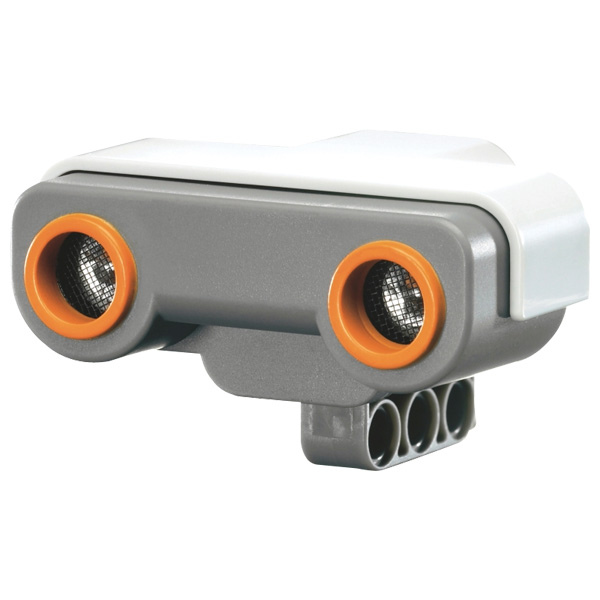
\includegraphics[width=.5\textwidth]{us}
\caption{Ultrasonisk sensor}
\label{sensor:ultrasonic_sensor}
\end{subfigure}
\begin{subfigure}[b]{.4\textwidth}
\centering
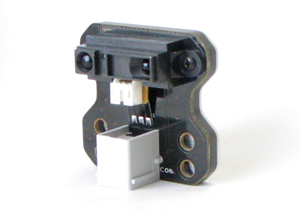
\includegraphics[width=.5\textwidth]{infrared_sensor}
\caption{Infrarød sensor}
\label{sensor:infraroed_sensor}
\end{subfigure}
\begin{subfigure}[b]{.4\textwidth}
\centering
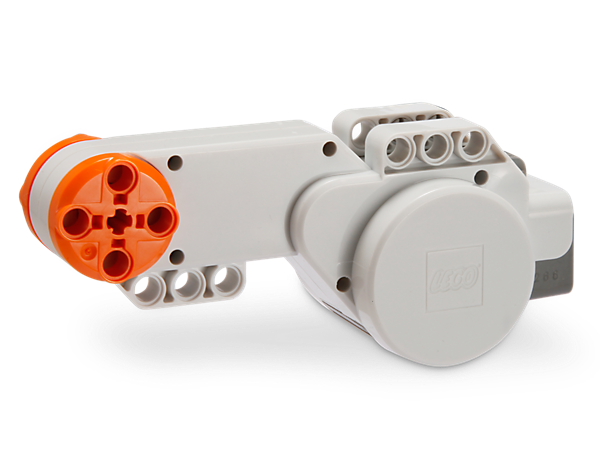
\includegraphics[width=.5\textwidth]{lego_motor}
\caption{Servomotor}
\label{sensor:servo_motor}
\end{subfigure}
\begin{subfigure}[b]{.4\textwidth}
\centering
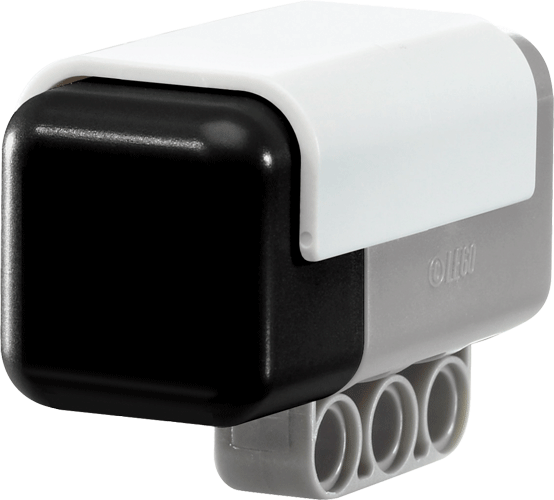
\includegraphics[width=.5\textwidth]{hitechnic_compass}
\caption{Kompas}
\label{sensor:compass}
\end{subfigure}
\end{figure}

\section{Afstandssensorer}
Dette afsnit beskriver testen af de to afstandssensorer, som kunne være interessante at montere på robotten.
For at afgøre hvilken der passer bedst til at løse problemet er de blevet testet.

Formålet med at teste disse sensorer er, at robotten skal have en måde at afgøre på, hvor langt der er til objekter omkring den.
Derfor vil disse tests undersøge følgende:
\begin{itemize}
\item Hvor nøjagtigt kan sensorerne bestemme afstanden til et objekt?
\item Hvilket interval kan der måles i, hvad er den minimale og maksiamle måleafstand?
\end{itemize}

\subsection{Ultrasonic Sensor}
Ultrasonic sensoren, som kan ses på \cref{sensor:ultrasonic_sensor}, er en sensor der kan måle afstand til objekter.

Det gøres ved at sende en lydbølge, hvorefter der beregnes hvor lang tid det tager for denne at ramme objektet, for derefter at blive reflekteret tilbage igen.
Sensoren måler afstanden i cm eller tommer.
Den maksimale afstand der kan måles er 255 cm med en præcision på $\pm$3 centimeter.
De bedste aflæsninger fås ved måling af store flade objekter med hård overflade, i modsætning til mindre objekter med rund og/eller blød overflade.\cite{nxt}

\subsubsection{Test}
Der er gennemført en mindre test af sensoren, for at finde ud af hvor nøjagtig den er.

Testen blev udført ved at lave en simpel konstruktion kun bestående af NXT og den ultrasoniske sensor.
Konstruktionen blev placeret i en række afstande fra en væg, hvor sensoreren var placeret vandret, pegende direkte på væggen.
Herefter blev sensoren aflæst, samtidig med at afstanden mellem væg og sensor blev målt med lineal.
Den samme test blev udført 3 gange.

\subsubsection{Resultater} Tabel med resultater fra forsøget kan ses i \cref{appendix:ultrasonisk}.

En graf-repræsentation af resultaterne kan ses i \cref{sensor:ultrasonic_resultat_diagram}.
Den røde linje indikerer det ideele resultat mens den blå, brune og grønne linje viser de resultaterne fra de tre test.
Det ses på grafen at de tre tests alle giver forkerte resultater når sensoren er mindre en 20 cm fra objektet.
Desuden kan det ses at der i test1 kun kunne måles op til 170 cm før der opstod usikkerhed, hvor de andre tests nåede 200 (test2) og 230 (test3) cm før der opstod større usikkerhed.
Generelt holder det som der bliver lovet, nemlig at der er en afvigelse på 3 cm på målingerne, men forsøget viser at der kun med sikkerhed kan måles mellem 20 og 170 cm.

\begin{figure}[h]
\centering
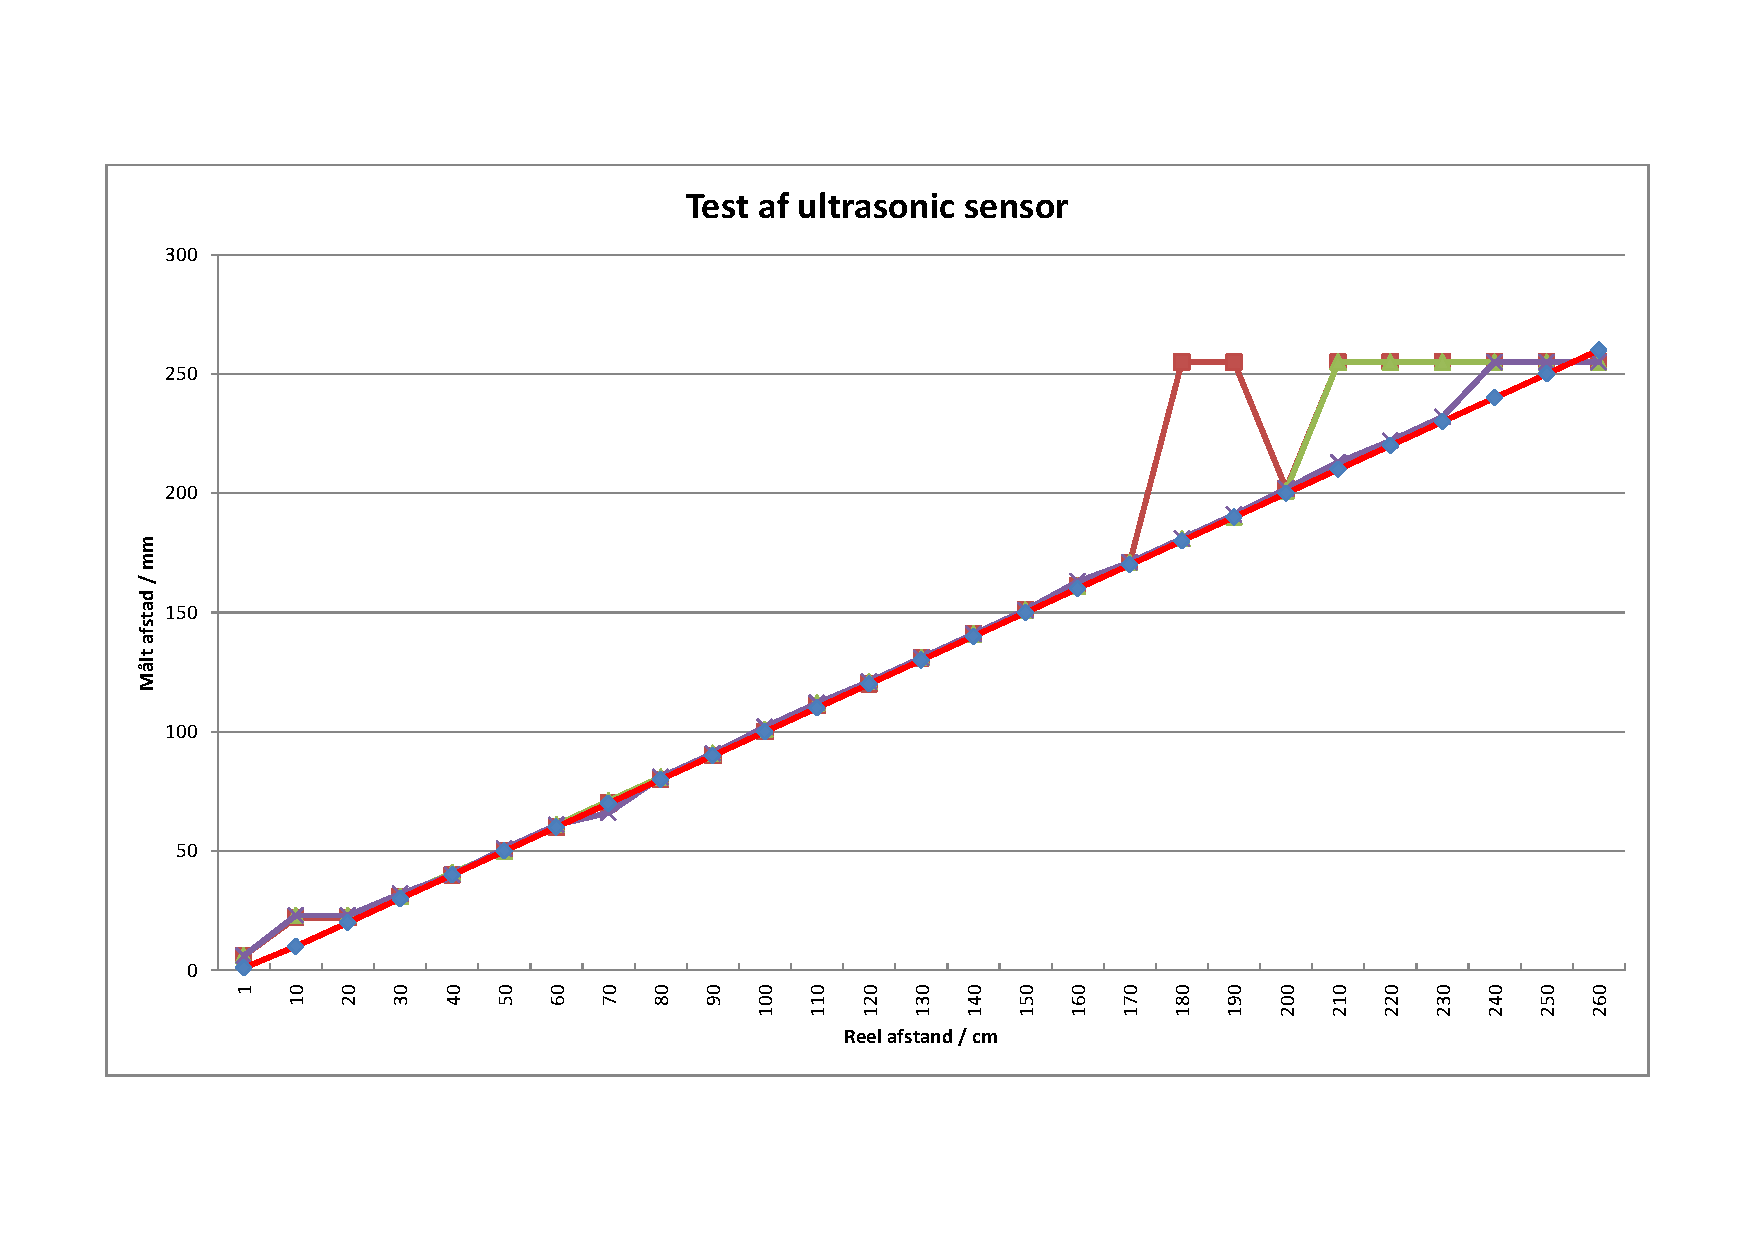
\includegraphics[clip=true, trim = 0cm 2.5cm 0cm 2.5cm,width=\textwidth]{ultrasonicchart}
\caption{Graf over forsøgsresultaterne fra testen af den ultrasoniske sensor}
\label{sensor:ultrasonic_resultat_diagram}
\end{figure}



\subsection{Infrarød Sensor}
Den infrarøde afstandssensor fra mindsensors.com, som kan ses på \cref{sensor:infraroed_sensor}, er en afstandssensor med høj præcision og måler afstande mellem 10 og 80 cm.
Sensoren virker som ultrasonisk sensoren, men sender et infrarødt signal i stedet for en ultrasonisk impuls.

\subsubsection{Test}
For at afprøve sensorens præcision og rækkevidde er der foretaget en test af sensoren.

Opstillingen brugt til udførelse af testen bestod af tre A4 ark spændt ud på gulvet ind til en væg. 
Papiret havde markeringer for hver 2 cm fra væggen.

Udførelsen af testen gik ud på at placere en NXT med påsat infrarød sensor ved hver indikator, for derefter at aflæse sensorens måling.
På denne måde blev afmålingen fra sensoren ved en given afstand holdt op imod den egentlige afstand til væggen, som afmålt på papiret.

\subsubsection{Resultater}

Resultaterne fra testen er præsenteret i \cref{appendix:infrared}. 
Disse resultater er sat op i et diagram i \cref{sensor:infrared_chart}.
Den røde graf er den reelle afstand, som aflæst på papiret/med lineal, mens de blå firkanter er målepunkter.
Den sorte graf er en lineær regression over måleresultaterne.

Ud fra grafen kan det ses at der er stor usikkerhed i starten og slutningen, hvilket næsten stemmer overens med den lovede rækkevidde på 10 til 80 cm.
De bedste resultater findes dog imellem 8cm og 56 cm. 
Mellem 8cm og 56cm er der maximalt 27 mm afvigelse fra det forventede, (forventet 500, målt 527).

\begin{figure}[h]
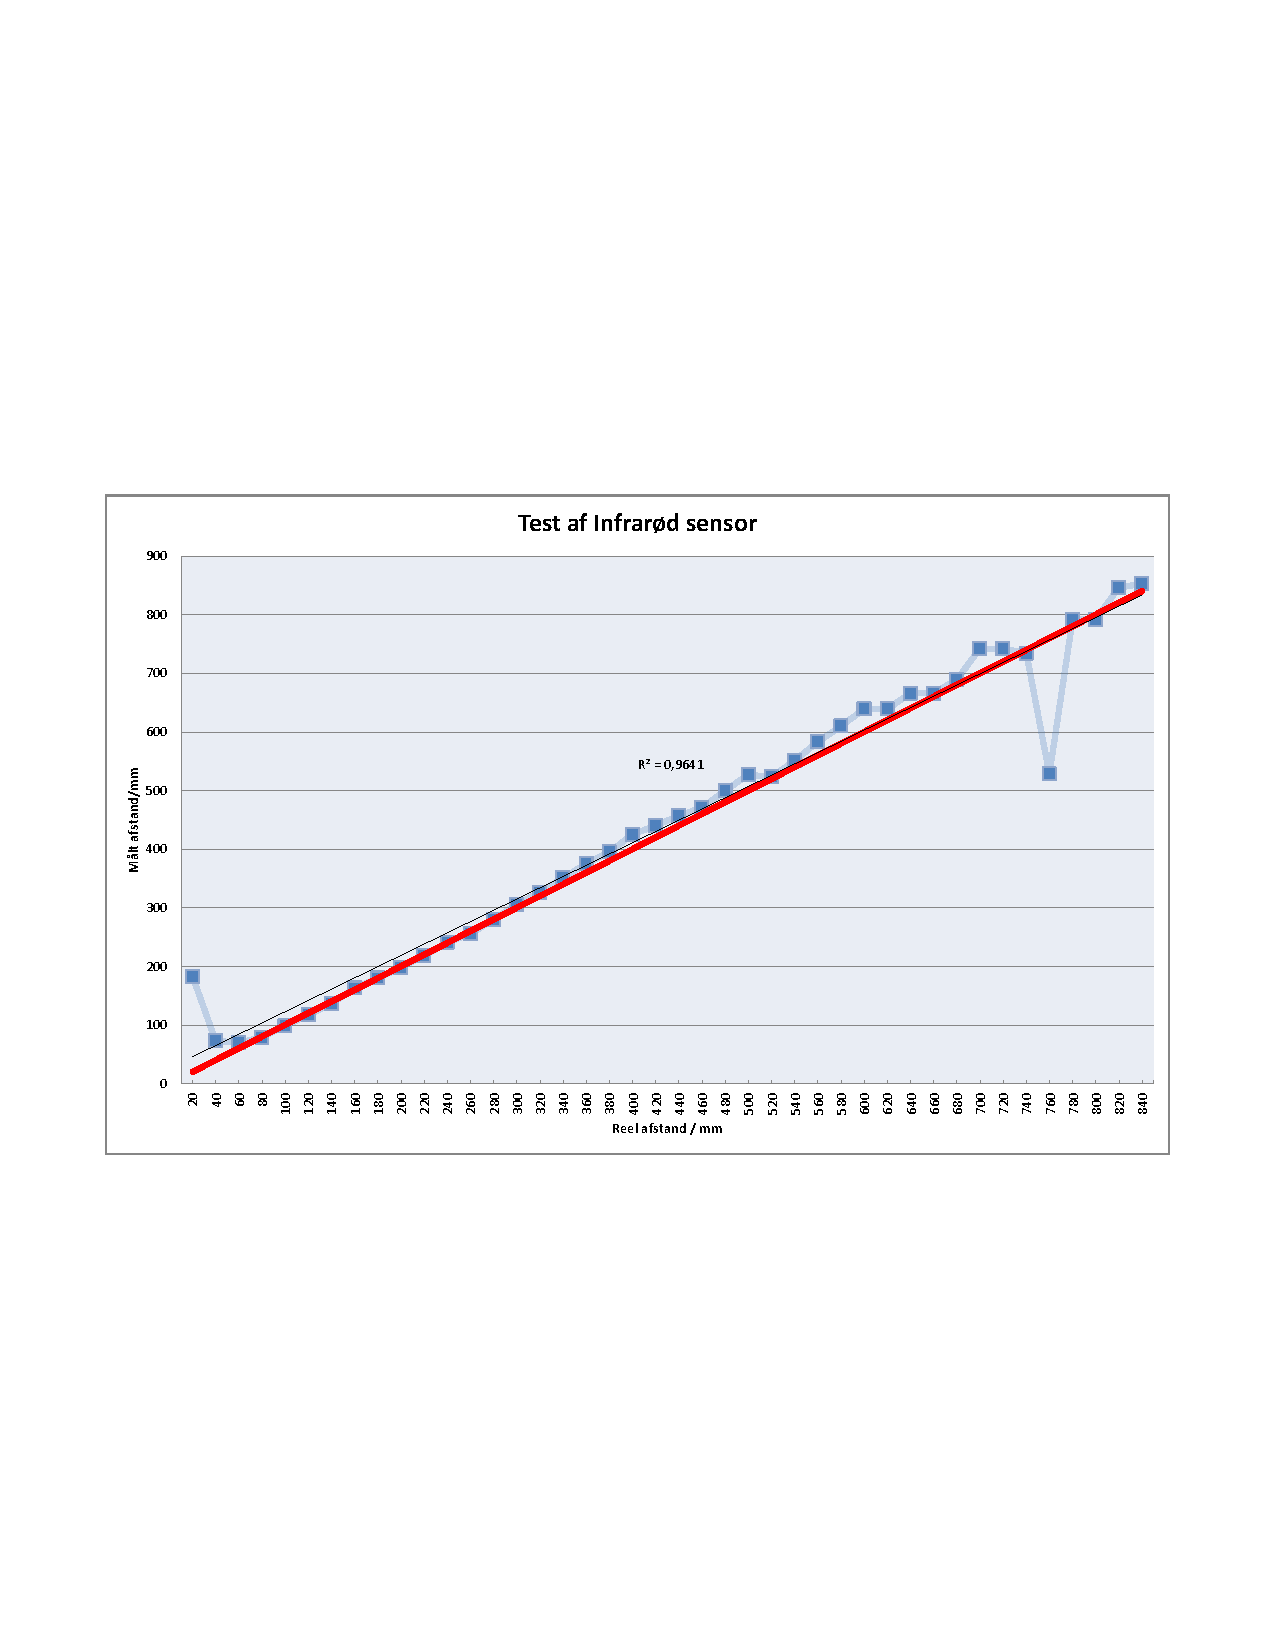
\includegraphics[clip=true, trim=0cm 8cm 0cm 8cm,width=\textwidth]{Infraredchart}
\caption{Graf over forsøgsresultaterne fra testen af den infrarøde sensor}
\label{sensor:infrared_chart}
\end{figure}

\subsection{Sammenligning af afstandssensorer}

Der er nu foretaget test af to forskellige afstandssensorer, den ultrasoniske sensor og den infrarøde sensor. 
Den ultrasoniske sensor var præcis med en afvigelse på $\pm$3 cm mellem 20 cm og 170 cm.
Den infrarøde sensor var præcis med afvigelse på $\pm$3 cm, mellem 10 cm og 56 cm.
Den infrarøde sensor angiver sine målinger med højere præcision, men da fejlmarginen er 3 cm anses den ikke som værende mere præcis end den ultrasoniske sensor.
I forhold til rækkevidden, måler den ultrasoniske længere væk end den infrarøde, mens den infrarøde sensor måler tættere på end den ultrasoniske.
Valget mellem de to sensorer står derfor på hvilket krav robotten har til rækkevidde.

\section{Motor}\label{sensorer:motorer}
Motoren der er testet her er fremstillet af \lego.
Den består af en rotationssensor, som måler omdrejningerne ved grader med en nøjagtighed på \'en grad ifølge \lego. 
Desuden gør denne sensor det også muligt at styre hvor meget kraft motoren skal køre med.
Køres der med flere motorer har NXT'en indbygget software, der gør det muligt at synkronisere disse, hvilket er smart hvis den ene motor skulle være stærkere eller svagere end den anden.\cite{tikNXT}
Motoren kan ses på \cref{sensor:servo_motor}.
\mikkel{Ovenstående skal skrives om - jeg nåede det bare ikke inden vi sendte til vejleder}

\subsection{Formål}
Formålet med denne test er at teste motorens nøjagtighed.
Hvis motoren ikke har høj nøjagtighed skal der tages højde for det når den moteres på robotten.

\subsection{Test}
For at bestemme motorens nøjagtighed i praksis, blev en test opstillet hvor to moterer roteres med et bestemt antal grader.
Motorernes egentlige rotation aflæses med vinkelmåler og holdes op mod den ønskede rotation, samt den rotation motorerne angiver at de har roteret.
Sidstenævnte fås ved at aflæse motorernes \lstinline[style=csharp]!TachoCount! egenskab.

\paragraph{Resultaterne} fra forsøget kan ses i \cref{appendix:motor_test}. 
\mikkel{Der er nogle fejl i dette afsnit som skal rettes efter vi har sendt til vejleder}
Af resultaterne kan vi bestemme den største afvigelse til +7 og -4 grader målt.
Tacho-værdien har en afvigelse på maksimalt +1 og -4 grader.
Dette stemmer ikke overens med de antagede $\pm$1 grad afvigelse.

+7 og +6 grader målt optræder kun en gang.
Ellers er den maksimale målte afvigelse $\pm$4 grader, men selvom vi antager at det er pga. unøjagtige målinger ved forsøgsudførelsen, er det stadig ikke $\pm$1 grad.
\stefan{Man kan ikke direkte aflæse afvigelserne fra tabellen}
\thilemann{Synes heller ikke meningen står helt klar}
Kigger vi på \cref{sensor:motor_sensor_diagram} kan vi se at målingerne ligger længst udenfor det optimale (sorte stiplede linje), hvilket er en god indikator på at det er bedre at benytte tacho-værdien.

\begin{figure}
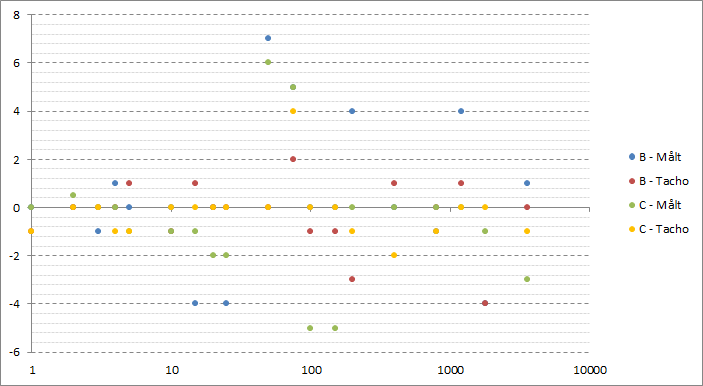
\includegraphics[width=\textwidth]{motor_diagram}
\caption{Afvigelser i test-resultaterne}
\label{sensor:motor_sensor_diagram}
\end{figure}

Desuden kan vi se på samme figur at motor b er meget mere unøjagtig end motor c.
Ideelt ville de to motorer give det samme resultat.

Dvs. den målte værdi har en afvigelse på $\pm$4 grader, mens tacho-værdien har en afvigelse på +1 og -4 grader, og at synkronisering af de to motrer ikke giver den ønskede effekt.

\section{HiTechnic NXT Compass Sensor}
Kompasset fra HiTechnic er et digitalt kompas der måler jordens magnetiske felt.
Kompasset kan returnere en værdi der repræsenterer kompassets nuværende orientering.
Ifølge HiTechnic er værdierne returneret fra kompasset præcise ned til 1 grad.
Kalibrering skulle desuden ikke være nødvendig.
Dog er det nødvendigt for at minimere forstyrrelser, at kompasset holdes 10-15 cm væk fra forstyrrende elementer, herunder \lego NXT og motorer.\cite{hitechnic_compass}

I \cref{kompas:precision} undersøges hvorvidt målinger fra kompasset kan leve op til disse oplysninger.

\subsection{Formål}
Formålet med denne test er at undersøge kompassets nøjagtighed.
Hvis kompasset har høj nøjagtighed kan det monteres på robotten og afgøre hvilken retning denne vender.

\subsection{Compass Sensor i \mindsqualls}
Til at styre denne sensor i \mindsqualls, skal der bruges en af de seperate klasser til HiTechnic sensorerne, som findes i namespacet \lstinline[style=csharp]!NXT.MindSqualls.HiTechnic!.
Til kompas sensoren anvendes klassen \lstinline[style=csharp]!HiTechnicCompassSensor!.

\subsubsection{Aflæsning af værdier}\label{kompas:reading}
Ved aflæsning af egenskaben \lstinline[style=csharp]!Heading! fra sensores klasse, gives et heltal mellem 0 og 359 der angiver kompassets orientering.
Det har været nødvendigt at ændre implementationen af \lstinline[style=csharp]!Heading!, da den oprindelige implementation ikke aflæste kompassets orientering ned til \'en grad.
Sensoren repræsenterer sin orientering på to forskellige måder.
Begge anvender to bytes.
Den ene metode beskriver afstanden vha. et 16-bit heltal.
Den anden (som var anvendt i implementationen af \lstinline[style=csharp]!Heading!) beskriver afstanden ved at lave den ene byte angive vinklen i intervaller af to grader.
Altså kunne de værdier der aflæses fra denne byte være 0-179, hvilket efterfølgende ganges med 2 for at få den egentlige værdi.
Hertil lægges værdien af den anden byte - der kan have værdien 0 eller 1.
I den oprindelige implementation af \lstinline[style=csharp]!Heading! er der ikke taget højde for denne ekstra værdi.
Dette er inddraget i test 3 i det følgende afsnit.

\subsection{Præcisionstest}\label{kompas:precision}
For at teste kompas sensoren, er målinger taget fra denne og holdt sammen med målinger foretaget med vinkelmåler.
Sammenligningen er sket ved at tage to målinger med kompasset, og sammenligne differencen med den værdi målt med vinkelmåler.
I forbindelse med test af sensoren blev der udført i alt tre tests:
\begin{enumerate}
\item Kompas monteret på robot med hjul
\item Kompas monteret på fast konstruktion
\item Gentagelse af test 2, med \textit{øget præcision}
\end{enumerate}
Den øgede præcision der beskrives her, dækker over en opdatering af \mindsqualls klassen \lstinline[style=csharp]!HiTechnicCompassSensor! der blev foretaget efter de første to tests.
Resultaterne fra de tre tests kan ses i tabellerne \ref{kompas:test1:table}, \ref{kompas:test2:table} og \ref{kompas:test3:table} på side \pageref{kompas:test1:table}.

Af resultaterne er der lavet et boksplot (\cref{kompas:boksplot}).
Plottet illustrerer den afvigelse der var fra de værdier der blev aflæst af kompasset, til de værdier der blev målt med vinkelmåler.
Prikkerne på plottet repræsenterer den gennemsnitlige afvigelse.

\begin{figure}[h]
\centering
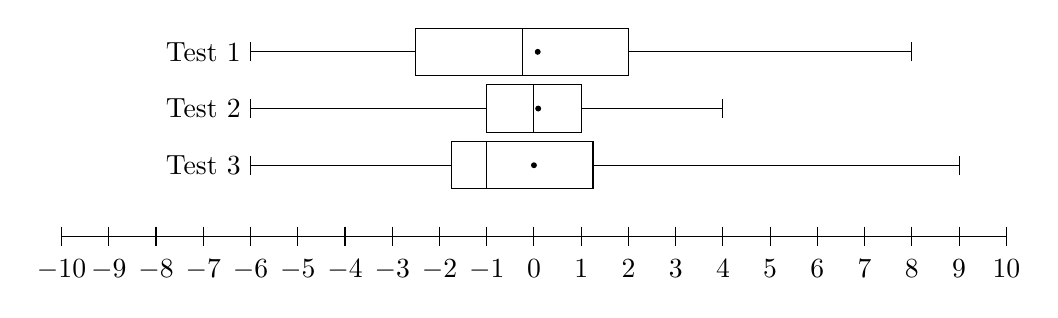
\begin{tikzpicture}[scale=0.6]
%Test 1
\draw (-2.5,3.4) rectangle (2,4.4); % Boks
\draw (-0.25,3.4) -- (-0.25,4.4); % Median streg
\draw (2,3.9) -- (8,3.9); % Fra øvre kvartil til maks
\draw (-2.5,3.9) -- (-6,3.9);% Fra nedre kvartil til min
\draw (8,3.7) -- (8,4.1); % Maksimum vertikal streg
\draw (-6,3.7) -- (-6,4.1); % Minimum vertikal streg
\node[left] at (-6,3.9) {Test 1};
\filldraw[color=black] (0.08,3.9) circle (0.05cm); % Gennemsnittet

%Test 2
\draw (-1,2.2) rectangle (1,3.2); % Boks
\draw (0,2.2) -- (0,3.2); % Median streg
\draw (1,2.7) -- (4,2.7); % Fra øvre kvartil til maks
\draw (-1,2.7) -- (-6,2.7);% Fra nedre kvartil til min
\draw (4,2.5) -- (4,2.9); % Maksimum vertikal streg
\draw (-6,2.5) -- (-6,2.9); % Minimum vertikal streg
\node[left] at (-6,2.7) {Test 2};
\filldraw[color=black] (0.09,2.7) circle (0.05cm); % Gennemsnittet

%Test 3
\draw (-1.75,1) rectangle (1.25,2); % Boks
\draw (-1,1) -- (-1,2); % Median streg
\draw (1.25,1.5) -- (9,1.5); % Fra øvre kvartil til maks
\draw (-1.75,1.5) -- (-6,1.5);% Fra nedre kvartil til min
\draw (9,1.3) -- (9,1.7); % Maksimum vertikal streg
\draw (-6,1.3) -- (-6,1.7); % Minimum vertikal streg
\node[left] at (-6,1.5) {Test 3};
\filldraw[color=black] (0.00,1.5) circle (0.05cm); % Gennemsnittet

% Linje med værdier
\draw (-10,0) -- (10,0);

% Tal på linje
\foreach \x in {-10,-9,...,10} {
	\draw (\x, 0.2) -- (\x, -0.2);
     \node[below] at (\x, -0.3) {$\x$};
}

\end{tikzpicture}
\caption{Boksplot for test af kompas.}
\label{kompas:boksplot}
\end{figure}

\subsubsection{Test 1: Monteret på robot}
Første forsøg blev udført med kompasset monteret ovenpå ultralyds-sensoren, for at holde en minimum-afstand på 15 cm fra brick og motorer.
Denne konstruktion var dog meget ustabil, da kompasset skulle være forholdsvist højt oppe ift. base-konstruktionen.

\subsubsection{Test 2: Monteret på stabil konstruktion}
Andet forsøg blev udført med kompasset monteret på en selvstændig og langt mere stabil konstruktion, for derved at undersøge om dette kunne forbedre resultaterne.

\subsubsection{Test 3: Forøget præcision (stabil konstruktion)}
Tredje forsøg var en gentagelse af det andet, efter implementationen af \lstinline[style=csharp]!Heading! blev opdateret.
Målingerne her skulle altså udtrykke en øget præcision i forhold til den forrige test.
Det er valgt at medtage de første to tests, da forbedringen af præcisionen højst kunne være \'en grad ved denne tredje test (se \textit{\cref{kompas:reading}: \nameref*{kompas:reading}}).
Altså en marginal forbedring i forhold til testresultaterne.

\subsubsection{Resultater}
Resultaterne kan ses i \cref{appendix:kompas_test}. Som det fremgår af \cref{kompas:boksplot} er den gennemsnitlige afvigelse i alle tests meget tæt på 0.
Altså ved vi at kompasset lave lige mange og lige store (i gennemsnit) udsving til begge sider, hvilket gør det sværere at kalibrere for sådanne udsving.
Samtidig viser plottet, at halvdelen af kompassets målinger er over 2-3$\dg$ ved siden af de egentlige målinger - med den største afvigelse på 9$\dg$.

Det har i testfasen vist sig, at kompasset er konsistent i dets målinger.
Dette betyder at der ikke kan opnås yderligere præcision ved at foretage flere målinger af samme grad.
Disse målinger vil ganske enkelt give samme resultat.

Det kan hermed konkluderes at kompas sensoren ikke har høj nok præcision til at kunne anvendes i projektet.

